% Test wrapper for example_workflow.tex (standalone compilation)
\documentclass[border=10pt]{standalone}
\usepackage[T1]{fontenc}
\usepackage{lmodern}
\usepackage{xcolor}
\usepackage{tikz}
\usepackage{amssymb}  % for \checkmark
\usetikzlibrary{shapes.geometric, arrows.meta, positioning, calc, fit, backgrounds, shadows}

% --- Colors ---
\definecolor{agentOrange}{RGB}{255, 240, 220}
\definecolor{agentCyan}{RGB}{225, 250, 250}
\definecolor{agentPurple}{RGB}{240, 230, 255}
\definecolor{agentTeal}{RGB}{220, 245, 245}
\definecolor{googleGray}{RGB}{240, 240, 240}
\definecolor{orchBlue}{RGB}{230, 240, 255}
\definecolor{planGreen}{RGB}{235, 255, 235}
\definecolor{failRed}{RGB}{255, 220, 220}
\definecolor{aliceblue}{RGB}{240, 248, 255}
\definecolor{stateBlue}{RGB}{235, 245, 255}
\definecolor{agentGreen}{RGB}{230, 255, 230}
\definecolor{agentRed}{RGB}{255, 230, 230}

% --- Icons ---
\newcommand{\iconDNA}[1]{\tikz[baseline=-3pt, scale=0.25]{\draw[#1, thick] (0,0) sin (0.5,0.5) cos (1,0) sin (1.5,-0.5) cos (2,0);\draw[#1, thick] (0,0) sin (0.5,-0.5) cos (1,0) sin (1.5,0.5) cos (2,0);}}
\newcommand{\iconGraph}[1]{\tikz[baseline=-3pt, scale=0.25]{\fill[#1] (0,0) circle (5pt) (1,0.5) circle (5pt) (1,-0.5) circle (5pt);\draw[#1, thick] (0,0)--(1,0.5) (0,0)--(1,-0.5) (1,0.5)--(1,-0.5);}}
\newcommand{\iconSearch}[1]{\tikz[baseline=-3pt, scale=0.25]{\draw[#1, thick] (0,0) circle (0.5cm);\draw[#1, very thick] (0.35,-0.35)--(0.7,-0.7);}}
\newcommand{\iconBulb}[1]{\tikz[baseline=-3pt, scale=0.25]{\draw[#1, thick, fill=white] (0,0) circle (0.5cm);\draw[#1] (-0.2,-0.4)--(-0.2,-0.7)--(0.2,-0.7)--(0.2,-0.4);\draw[#1] (0,0)--(0,0.3) (0,0)--(0.3,0.3) (0,0)--(-0.3,0.3);}}
\newcommand{\iconUser}[1]{\tikz[baseline=-3pt, scale=0.25]{\fill[#1] (0,0.5) circle (0.35cm);\fill[#1] (0,-0.1) ellipse (0.6cm and 0.3cm);}}
\newcommand{\iconBrain}[1]{\tikz[baseline=-3pt, scale=0.25]{\draw[#1, thick, fill=white] (0,0) ellipse (0.7cm and 0.5cm);\draw[#1] (-0.3,0)--(0.3,0) (0,-0.3)--(0,0.3);}}
\newcommand{\iconGears}[1]{\tikz[baseline=-3pt, scale=0.25]{\draw[#1, thick, fill=white] (0,0) circle (0.5cm);\draw[#1, dashed] (0,0) circle (0.35cm);}}
\newcommand{\iconCycle}[1]{\tikz[baseline=-3pt, scale=0.25]{\draw[#1, thick, ->] (0,0.4) arc (90:0:0.4);\draw[#1, thick, ->] (0,-0.4) arc (270:180:0.4);}}
\newcommand{\iconRobot}[1]{\tikz[baseline=-3pt, scale=0.25]{\draw[#1, thick, fill=white] (-0.5,-0.4) rectangle (0.5,0.4);\fill[#1] (-0.2,0) circle (2pt) (0.2,0) circle (2pt);\draw[#1] (0,0.4)--(0,0.7) circle (2pt);}}
\newcommand{\iconDoc}[1]{\tikz[baseline=-3pt, scale=0.25]{\draw[#1, thick, fill=white] (-0.3,-0.5) rectangle (0.3,0.5);\draw[#1] (-0.15,0.2)--(0.15,0.2) (-0.15,0)--(0.15,0) (-0.15,-0.2)--(0.15,-0.2);}}

% --- TikZ styles used by the workflow diagram ---
\tikzset{
    agentbox/.style={
        rectangle, rounded corners=6pt, draw=gray!30, thick,
        minimum width=7.5cm, minimum height=2.4cm, align=left,
        inner sep=6pt, drop shadow={opacity=0.10}
    },
    database/.style={
        cylinder, shape border rotate=90, draw=gray!30,
        minimum width=0.8cm, minimum height=1.0cm,
        font=\tiny\bfseries, align=center
    },
    statearrow/.style={->, >=latex, thick, draw=blue!30}
}

\usepackage{capt-of}  % provides \captionof without needing float

% Neutralize figure env for standalone
\renewenvironment{figure}[1][]{}{}
\renewcommand{\resizebox}[3]{#3}
\renewcommand{\caption}[2][]{}

\begin{document}
% ============================================================
% Example Workflow Diagram — Alzheimer's Disease Run
% Fragment: paste into main document via % ============================================================
% Example Workflow Diagram — Alzheimer's Disease Run
% Fragment: paste into main document via % ============================================================
% Example Workflow Diagram — Alzheimer's Disease Run
% Fragment: paste into main document via \input{figs/example_workflow}
% Requires preamble: agentbox, database, statearrow styles;
%   all icon commands; colors agentOrange/Cyan/Purple/Teal,
%   googleGray, stateBlue, aliceblue, agentGreen, \iconDoc.
% ============================================================

\begin{figure}[p]
\centering
\resizebox{\textwidth}{!}{%
    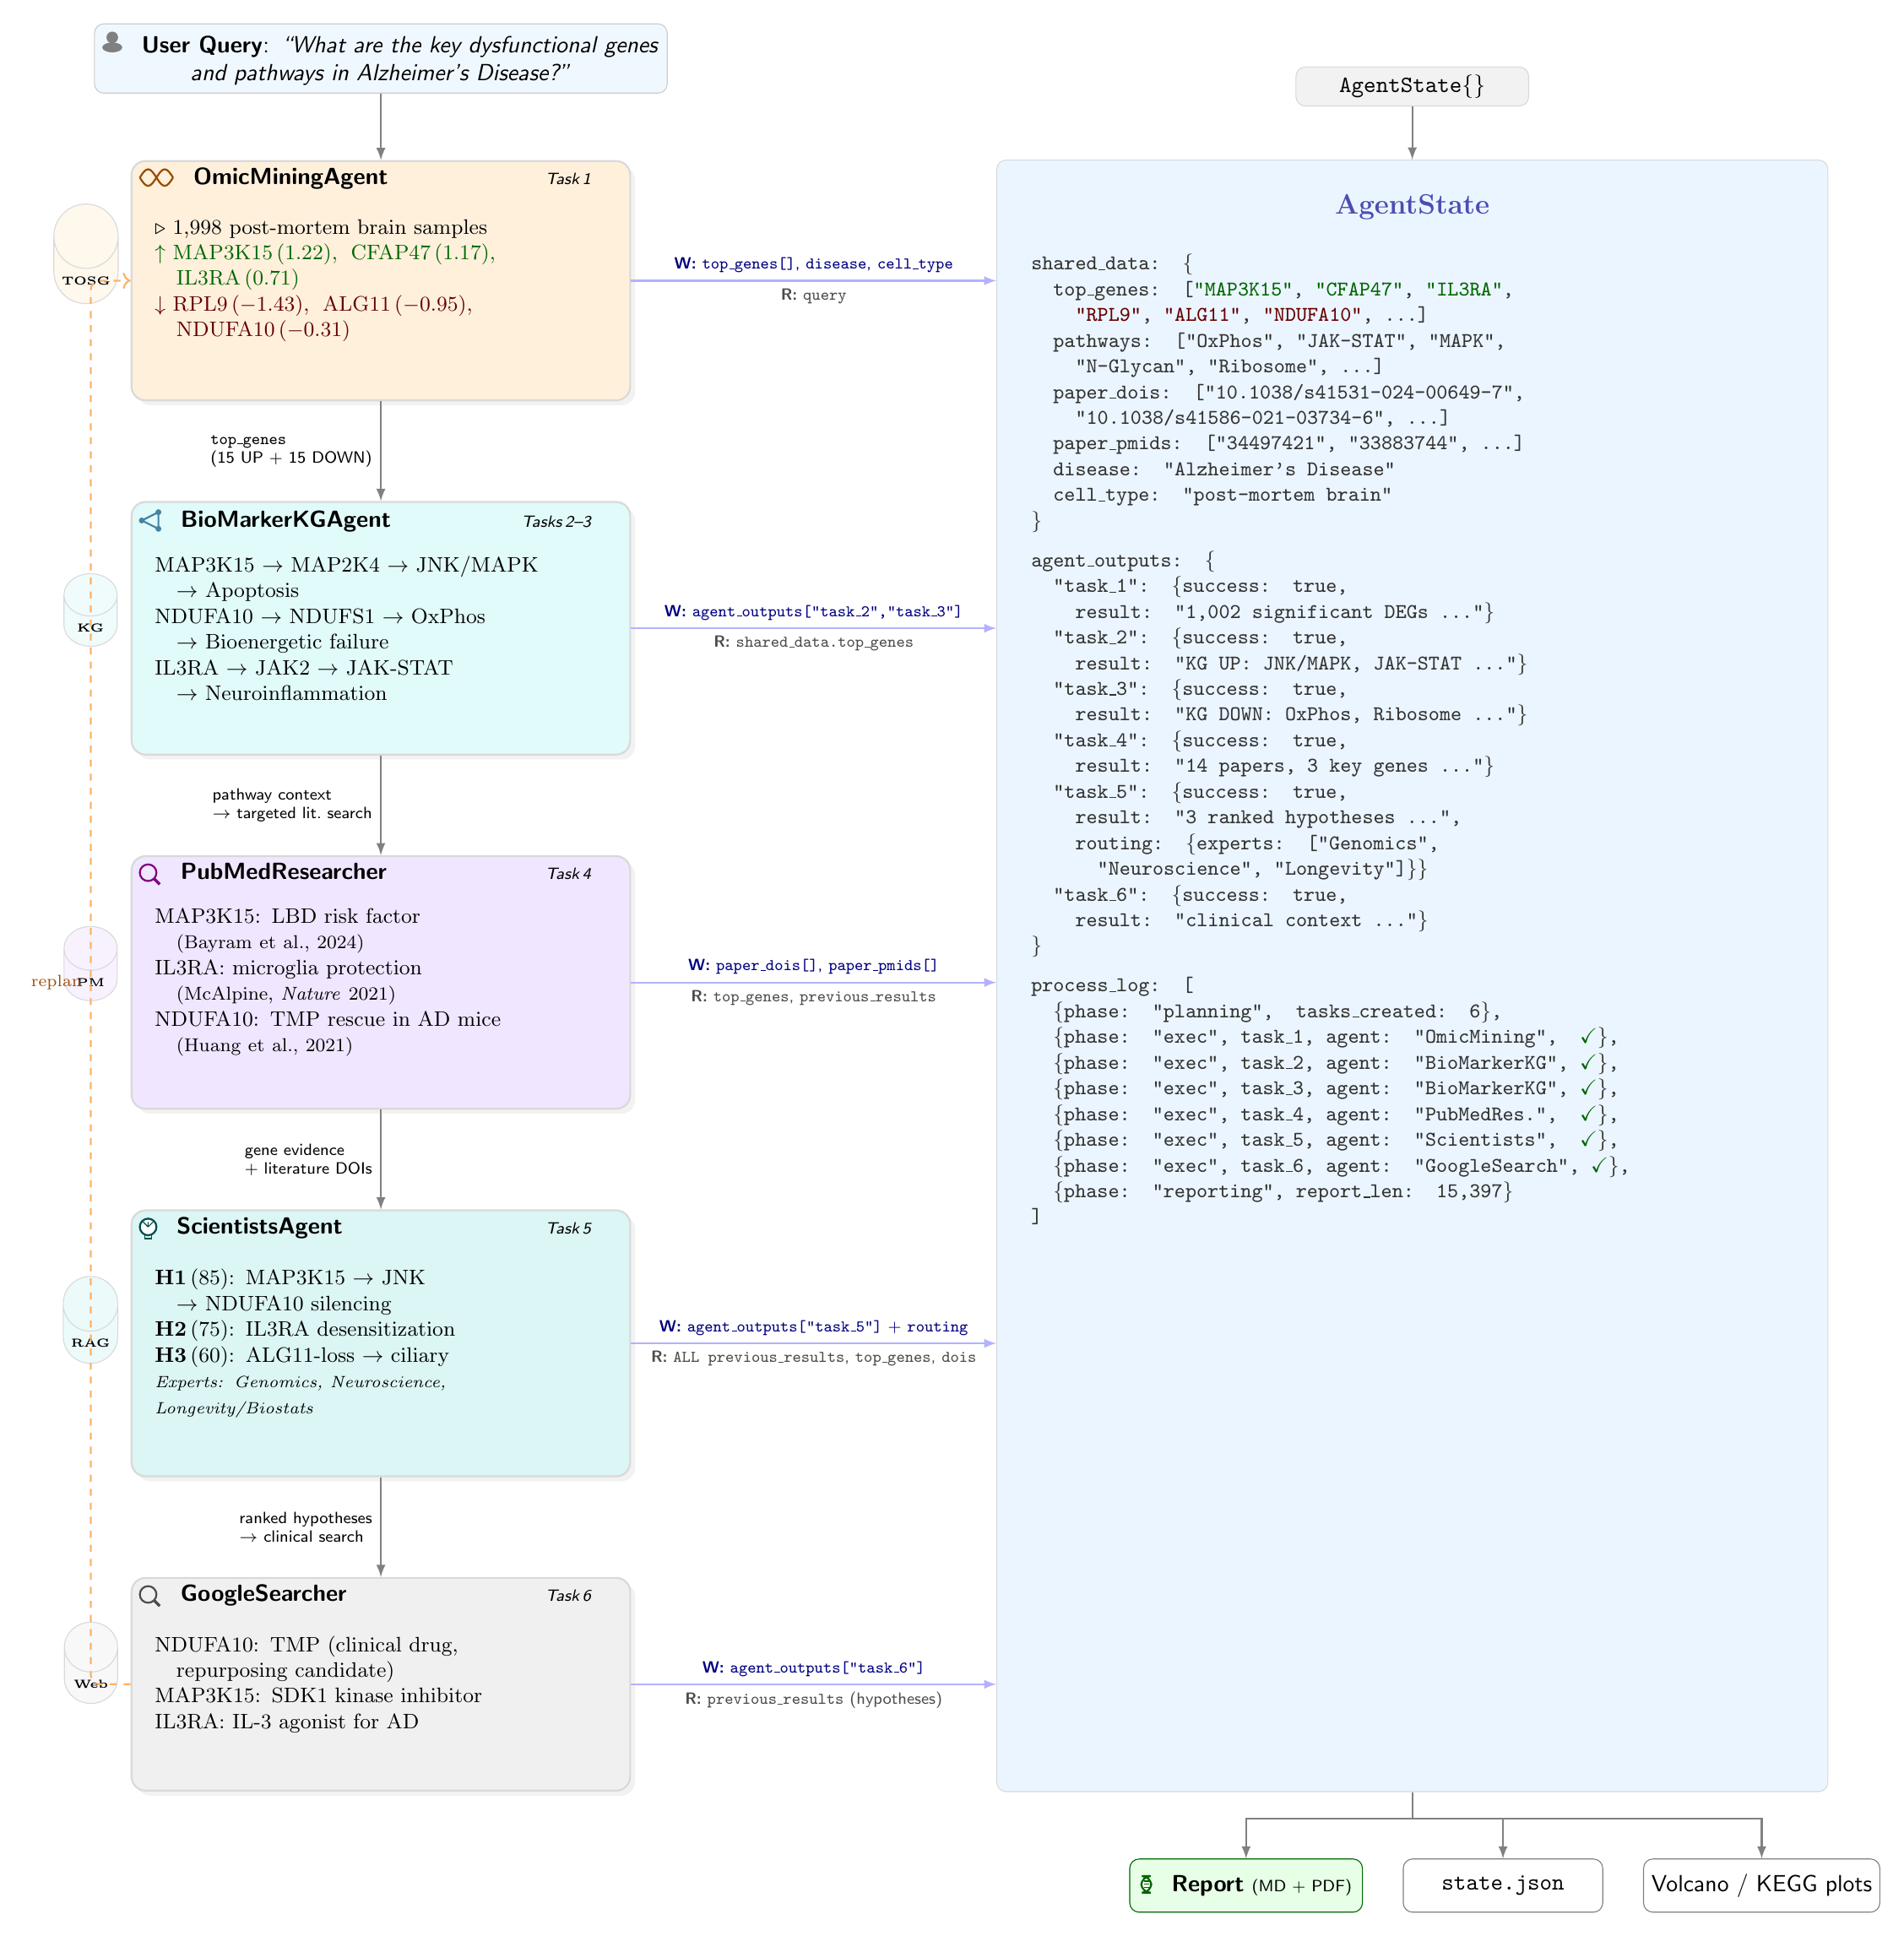
\begin{tikzpicture}[node distance=0.6cm and 1.5cm, font=\sffamily,
        % annotation styles for read/write labels
        wlabel/.style={font=\scriptsize\sffamily, text=blue!50!black, align=left, inner sep=1pt},
        rlabel/.style={font=\scriptsize\sffamily, text=gray!60!black, align=left, inner sep=1pt},
        flowlabel/.style={font=\scriptsize\sffamily, align=left}
    ]

    % ================= LEFT COLUMN: AGENTS =================

    % 1. Input
    \node[draw=gray!40, fill=aliceblue, rounded corners,
          minimum width=6.5cm, minimum height=1.0cm, align=center] (query)
        {\iconUser{gray} \enskip \textbf{User Query}:
         \textit{``What are the key dysfunctional genes}\\
         \textit{and pathways in Alzheimer's Disease?''}};

    % 2. OmicMiningAgent  (Task 1)
    \node[agentbox, fill=agentOrange, minimum height=3.6cm, below=1.0cm of query] (omic) {};
    \node[anchor=north west, text width=6.8cm] at (omic.north west)
        {\iconDNA{orange!60!black} \enskip \textbf{OmicMiningAgent}
         \hfill {\scriptsize\itshape Task\,1}};
    \node[anchor=center, font=\small, align=left, text width=6.8cm] at (omic.center) {
        $\triangleright$ 1{,}998 post-mortem brain samples\\
        \textcolor{green!40!black}{$\uparrow$ MAP3K15\,(1.22),\; CFAP47\,(1.17),}\\
        \textcolor{green!40!black}{\quad IL3RA\,(0.71)}\\
        \textcolor{red!40!black}{$\downarrow$ RPL9\,($-$1.43),\; ALG11\,($-$0.95),}\\
        \textcolor{red!40!black}{\quad NDUFA10\,($-$0.31)}
    };
    \node[database, fill=agentOrange!50, left=0.2cm of omic] (db1) {TOSG};

    % 3. BioMarkerKGAgent  (Tasks 2–3)
    \node[agentbox, fill=agentCyan, minimum height=3.8cm, below=1.5cm of omic] (kg) {};
    \node[anchor=north west, text width=6.8cm] at (kg.north west)
        {\iconGraph{cyan!60!black} \enskip \textbf{BioMarkerKGAgent}
         \hfill {\scriptsize\itshape Tasks\,2--3}};
    \node[anchor=center, font=\small, align=left, text width=6.8cm] at (kg.center) {
        MAP3K15 $\rightarrow$ MAP2K4 $\rightarrow$ JNK/MAPK\\
        \quad $\rightarrow$ Apoptosis\\
        NDUFA10 $\rightarrow$ NDUFS1 $\rightarrow$ OxPhos\\
        \quad $\rightarrow$ Bioenergetic failure\\
        IL3RA $\rightarrow$ JAK2 $\rightarrow$ JAK-STAT\\
        \quad $\rightarrow$ Neuroinflammation
    };
    \node[database, fill=agentCyan!50, left=0.2cm of kg] (db2) {KG};

    % 4. PubMedResearcher  (Task 4)
    \node[agentbox, fill=agentPurple, minimum height=3.8cm, below=1.5cm of kg] (pubmed) {};
    \node[anchor=north west, text width=6.8cm] at (pubmed.north west)
        {\iconSearch{violet} \enskip \textbf{PubMedResearcher}
         \hfill {\scriptsize\itshape Task\,4}};
    \node[anchor=center, font=\small, align=left, text width=6.8cm] at (pubmed.center) {
        MAP3K15: LBD risk factor\\
        \quad {\footnotesize(Bayram et al., 2024)}\\
        IL3RA: microglia protection\\
        \quad {\footnotesize(McAlpine, \textit{Nature} 2021)}\\
        NDUFA10: TMP rescue in AD mice\\
        \quad {\footnotesize(Huang et al., 2021)}
    };
    \node[database, fill=agentPurple!50, left=0.2cm of pubmed] (db3) {PM};

    % 5. ScientistsAgent  (Task 5 — multi-expert)
    \node[agentbox, fill=agentTeal, minimum height=4.0cm, below=1.5cm of pubmed] (scientist) {};
    \node[anchor=north west, text width=6.8cm] at (scientist.north west)
        {\iconBulb{teal!60!black} \enskip \textbf{ScientistsAgent}
         \hfill {\scriptsize\itshape Task\,5}};
    \node[anchor=center, font=\small, align=left, text width=6.8cm] at (scientist.center) {
        \textbf{H1}\,(85): MAP3K15 $\rightarrow$ JNK\\
        \quad $\rightarrow$ NDUFA10 silencing\\
        \textbf{H2}\,(75): IL3RA desensitization\\
        \textbf{H3}\,(60): ALG11-loss $\rightarrow$ ciliary\\
        {\scriptsize\itshape Experts: Genomics, Neuroscience,}\\
        {\scriptsize\itshape Longevity/Biostats}
    };
    \node[database, fill=agentTeal!50, left=0.2cm of scientist] (db4) {RAG};

    % 6. GoogleSearcher  (Task 6)
    \node[agentbox, fill=googleGray, minimum height=3.2cm, below=1.5cm of scientist] (google) {};
    \node[anchor=north west, text width=6.8cm] at (google.north west)
        {\iconSearch{gray!60!black} \enskip \textbf{GoogleSearcher}
         \hfill {\scriptsize\itshape Task\,6}};
    \node[anchor=center, font=\small, align=left, text width=6.8cm] at (google.center) {
        NDUFA10: TMP (clinical drug,\\
        \quad repurposing candidate)\\
        MAP3K15: SDK1 kinase inhibitor\\
        IL3RA: IL-3 agonist for AD
    };
    \node[database, fill=googleGray!50, left=0.2cm of google] (db5) {Web};


    % ================= RIGHT COLUMN: AgentState =================

    \node[draw=gray!30, fill=stateBlue, rounded corners, inner sep=0pt,
          fit={($(omic.north east)+(5.5cm,0)$) ($(google.south east)+(18.0cm,0)$)}]
          (statebox) {};

    % Header
    \node[anchor=north, font=\large\bfseries, color=blue!40!gray, yshift=-0.4cm]
        at (statebox.north) {AgentState};

    % State Content — real AD-test data
    \node[anchor=north west, align=left, font=\ttfamily\small,
          text=gray!40!black] at ($(statebox.north west) + (0.4cm, -1.3cm)$) {%
shared\_data: \{\\
\ \ top\_genes: [%
\textcolor{green!40!black}{"MAP3K15"}, %
\textcolor{green!40!black}{"CFAP47"}, %
\textcolor{green!40!black}{"IL3RA"},\\
\ \ \ \ %
\textcolor{red!40!black}{"RPL9"}, %
\textcolor{red!40!black}{"ALG11"}, %
\textcolor{red!40!black}{"NDUFA10"}, ...]\\
\ \ pathways: ["OxPhos", "JAK-STAT", "MAPK",\\
\ \ \ \ "N-Glycan", "Ribosome", ...]\\
\ \ paper\_dois: ["10.1038/s41531-024-00649-7",\\
\ \ \ \ "10.1038/s41586-021-03734-6", ...]\\
\ \ paper\_pmids: ["34497421", "33883744", ...]\\
\ \ disease: "Alzheimer's Disease"\\
\ \ cell\_type: "post-mortem brain"\\
\}\\[6pt]
agent\_outputs: \{\\
\ \ "task\_1": \{success: true,\\
\ \ \ \ result: "1{,}002 significant DEGs ..."\}\\
\ \ "task\_2": \{success: true,\\
\ \ \ \ result: "KG UP: JNK/MAPK, JAK-STAT ..."\}\\
\ \ "task\_3": \{success: true,\\
\ \ \ \ result: "KG DOWN: OxPhos, Ribosome ..."\}\\
\ \ "task\_4": \{success: true,\\
\ \ \ \ result: "14 papers, 3 key genes ..."\}\\
\ \ "task\_5": \{success: true,\\
\ \ \ \ result: "3 ranked hypotheses ...",\\
\ \ \ \ routing: \{experts: ["Genomics",\\
\ \ \ \ \ \ "Neuroscience", "Longevity"]\}\}\\
\ \ "task\_6": \{success: true,\\
\ \ \ \ result: "clinical context ..."\}\\
\}\\[6pt]
process\_log: [\\
\ \ \{phase: "planning",\ \ tasks\_created: 6\},\\
\ \ \{phase: "exec", task\_1, agent: "OmicMining",\quad \textcolor{green!40!black}{\checkmark}\},\\
\ \ \{phase: "exec", task\_2, agent: "BioMarkerKG",\ \textcolor{green!40!black}{\checkmark}\},\\
\ \ \{phase: "exec", task\_3, agent: "BioMarkerKG",\ \textcolor{green!40!black}{\checkmark}\},\\
\ \ \{phase: "exec", task\_4, agent: "PubMedRes.",\ \ \textcolor{green!40!black}{\checkmark}\},\\
\ \ \{phase: "exec", task\_5, agent: "Scientists",\ \ \textcolor{green!40!black}{\checkmark}\},\\
\ \ \{phase: "exec", task\_6, agent: "GoogleSearch", \textcolor{green!40!black}{\checkmark}\},\\
\ \ \{phase: "reporting", report\_len: 15{,}397\}\\
]
    };

    % Initial State Input
    \node[draw=gray!30, fill=gray!10, rounded corners,
          above=0.8cm of statebox, minimum width=3.5cm] (initstate)
        {\texttt{AgentState\{\}}};
    \draw[->, >=latex, thick, draw=gray] (initstate) -- (statebox);


    % ================= VERTICAL FLOW (data dependencies) =================
    % Labels on LEFT to avoid collision with horizontal read/write annotations

    \draw[->, >=latex, thick, draw=gray] (query) -- (omic);

    \draw[->, >=latex, thick, draw=gray] (omic) --
        node[left, flowlabel]
            {\texttt{top\_genes}\\{\scriptsize(15 UP + 15 DOWN)}} (kg);

    \draw[->, >=latex, thick, draw=gray] (kg) --
        node[left, flowlabel]
            {pathway context\\{\scriptsize$\rightarrow$ targeted lit.\ search}} (pubmed);

    \draw[->, >=latex, thick, draw=gray] (pubmed) --
        node[left, flowlabel]
            {gene evidence\\{\scriptsize+ literature DOIs}} (scientist);

    \draw[->, >=latex, thick, draw=gray] (scientist) --
        node[left, flowlabel]
            {ranked hypotheses\\{\scriptsize$\rightarrow$ clinical search}} (google);


    % ================= HORIZONTAL STATE ARROWS (read/write) =================

    % OmicMiningAgent → State
    \draw[statearrow] (omic.east) -- (omic.east -| statebox.west)
        node[midway, above=2pt, wlabel]
            {\textbf{W:} \texttt{top\_genes[]}, \texttt{disease}, \texttt{cell\_type}}
        node[midway, below=2pt, rlabel]
            {\textbf{R:} \texttt{query}};

    % BioMarkerKGAgent → State
    \draw[statearrow] (kg.east) -- (kg.east -| statebox.west)
        node[midway, above=2pt, wlabel]
            {\textbf{W:} \texttt{agent\_outputs["task\_2","task\_3"]}}
        node[midway, below=2pt, rlabel]
            {\textbf{R:} \texttt{shared\_data.top\_genes}};

    % PubMedResearcher → State
    \draw[statearrow] (pubmed.east) -- (pubmed.east -| statebox.west)
        node[midway, above=2pt, wlabel]
            {\textbf{W:} \texttt{paper\_dois[]}, \texttt{paper\_pmids[]}}
        node[midway, below=2pt, rlabel]
            {\textbf{R:} \texttt{top\_genes}, \texttt{previous\_results}};

    % ScientistsAgent → State
    \draw[statearrow] (scientist.east) -- (scientist.east -| statebox.west)
        node[midway, above=2pt, wlabel]
            {\textbf{W:} \texttt{agent\_outputs["task\_5"]} + \texttt{routing}}
        node[midway, below=2pt, rlabel]
            {\textbf{R:} \texttt{ALL previous\_results}, \texttt{top\_genes}, \texttt{dois}};

    % GoogleSearcher → State
    \draw[statearrow] (google.east) -- (google.east -| statebox.west)
        node[midway, above=2pt, wlabel]
            {\textbf{W:} \texttt{agent\_outputs["task\_6"]}}
        node[midway, below=2pt, rlabel]
            {\textbf{R:} \texttt{previous\_results} (hypotheses)};


    % ================= REPLAN LOOP =================
    \draw[->, dashed, draw=orange!60, thick, rounded corners]
        (google.west) -- ++(-0.6,0) |-
        node[pos=0.25, left, font=\scriptsize, color=orange!60!black] {replan}
        (omic.west);


    % ================= OUTPUTS =================

    \node[draw=green!40!black, fill=agentGreen, rounded corners,
          below=1.0cm of statebox, xshift=-2.5cm,
          minimum width=3.5cm, minimum height=0.8cm] (report)
        {\iconDoc{green!40!black} \enskip \textbf{Report}
         {\scriptsize(MD + PDF)}};

    \node[draw=gray, fill=white, rounded corners,
          right=0.6cm of report,
          minimum width=3.0cm, minimum height=0.8cm] (json)
        {\texttt{state.json}};

    \node[draw=gray, fill=white, rounded corners,
          right=0.6cm of json,
          minimum width=3.0cm, minimum height=0.8cm] (plots)
        {Volcano / KEGG plots};

    \draw[->, >=latex, thick, draw=gray]
        (statebox.south) -- ++(0,-0.4) -| (report.north);
    \draw[->, >=latex, thick, draw=gray]
        (statebox.south) -- ++(0,-0.4) -| (json.north);
    \draw[->, >=latex, thick, draw=gray]
        (statebox.south) -- ++(0,-0.4) -| (plots.north);

    \end{tikzpicture}%
}% end resizebox
\caption{Example agent workflow for an Alzheimer's Disease query using the
OmniCellAgent system.  The Planner decomposes the query into six sequential
tasks; each sub-agent receives the accumulated \texttt{AgentState} and writes
its outputs back.
\textbf{Read/write annotations} on each horizontal arrow show the specific
state fields consumed and produced: OmicMiningAgent populates
\texttt{top\_genes} (1{,}002 DEGs from 1{,}998 post-mortem brain samples),
BioMarkerKGAgent maps those genes to pathways via PrimeKG,
PubMedResearcher adds literature DOIs for the top hits, ScientistsAgent
routes to three domain experts (Genomics, Neuroscience, Longevity/Biostats)
and synthesises ranked mechanistic hypotheses, and GoogleSearcher assesses
translational viability (e.g.\ TMP for NDUFA10 rescue, SDK1 for MAP3K15
inhibition).  The downward arrows indicate how each step leverages results
from the preceding step---enabling progressively deeper reasoning that
mirrors the workflow of a human research team.}
\label{fig:workflow-example}
\end{figure}

% Requires preamble: agentbox, database, statearrow styles;
%   all icon commands; colors agentOrange/Cyan/Purple/Teal,
%   googleGray, stateBlue, aliceblue, agentGreen, \iconDoc.
% ============================================================

\begin{figure}[p]
\centering
\resizebox{\textwidth}{!}{%
    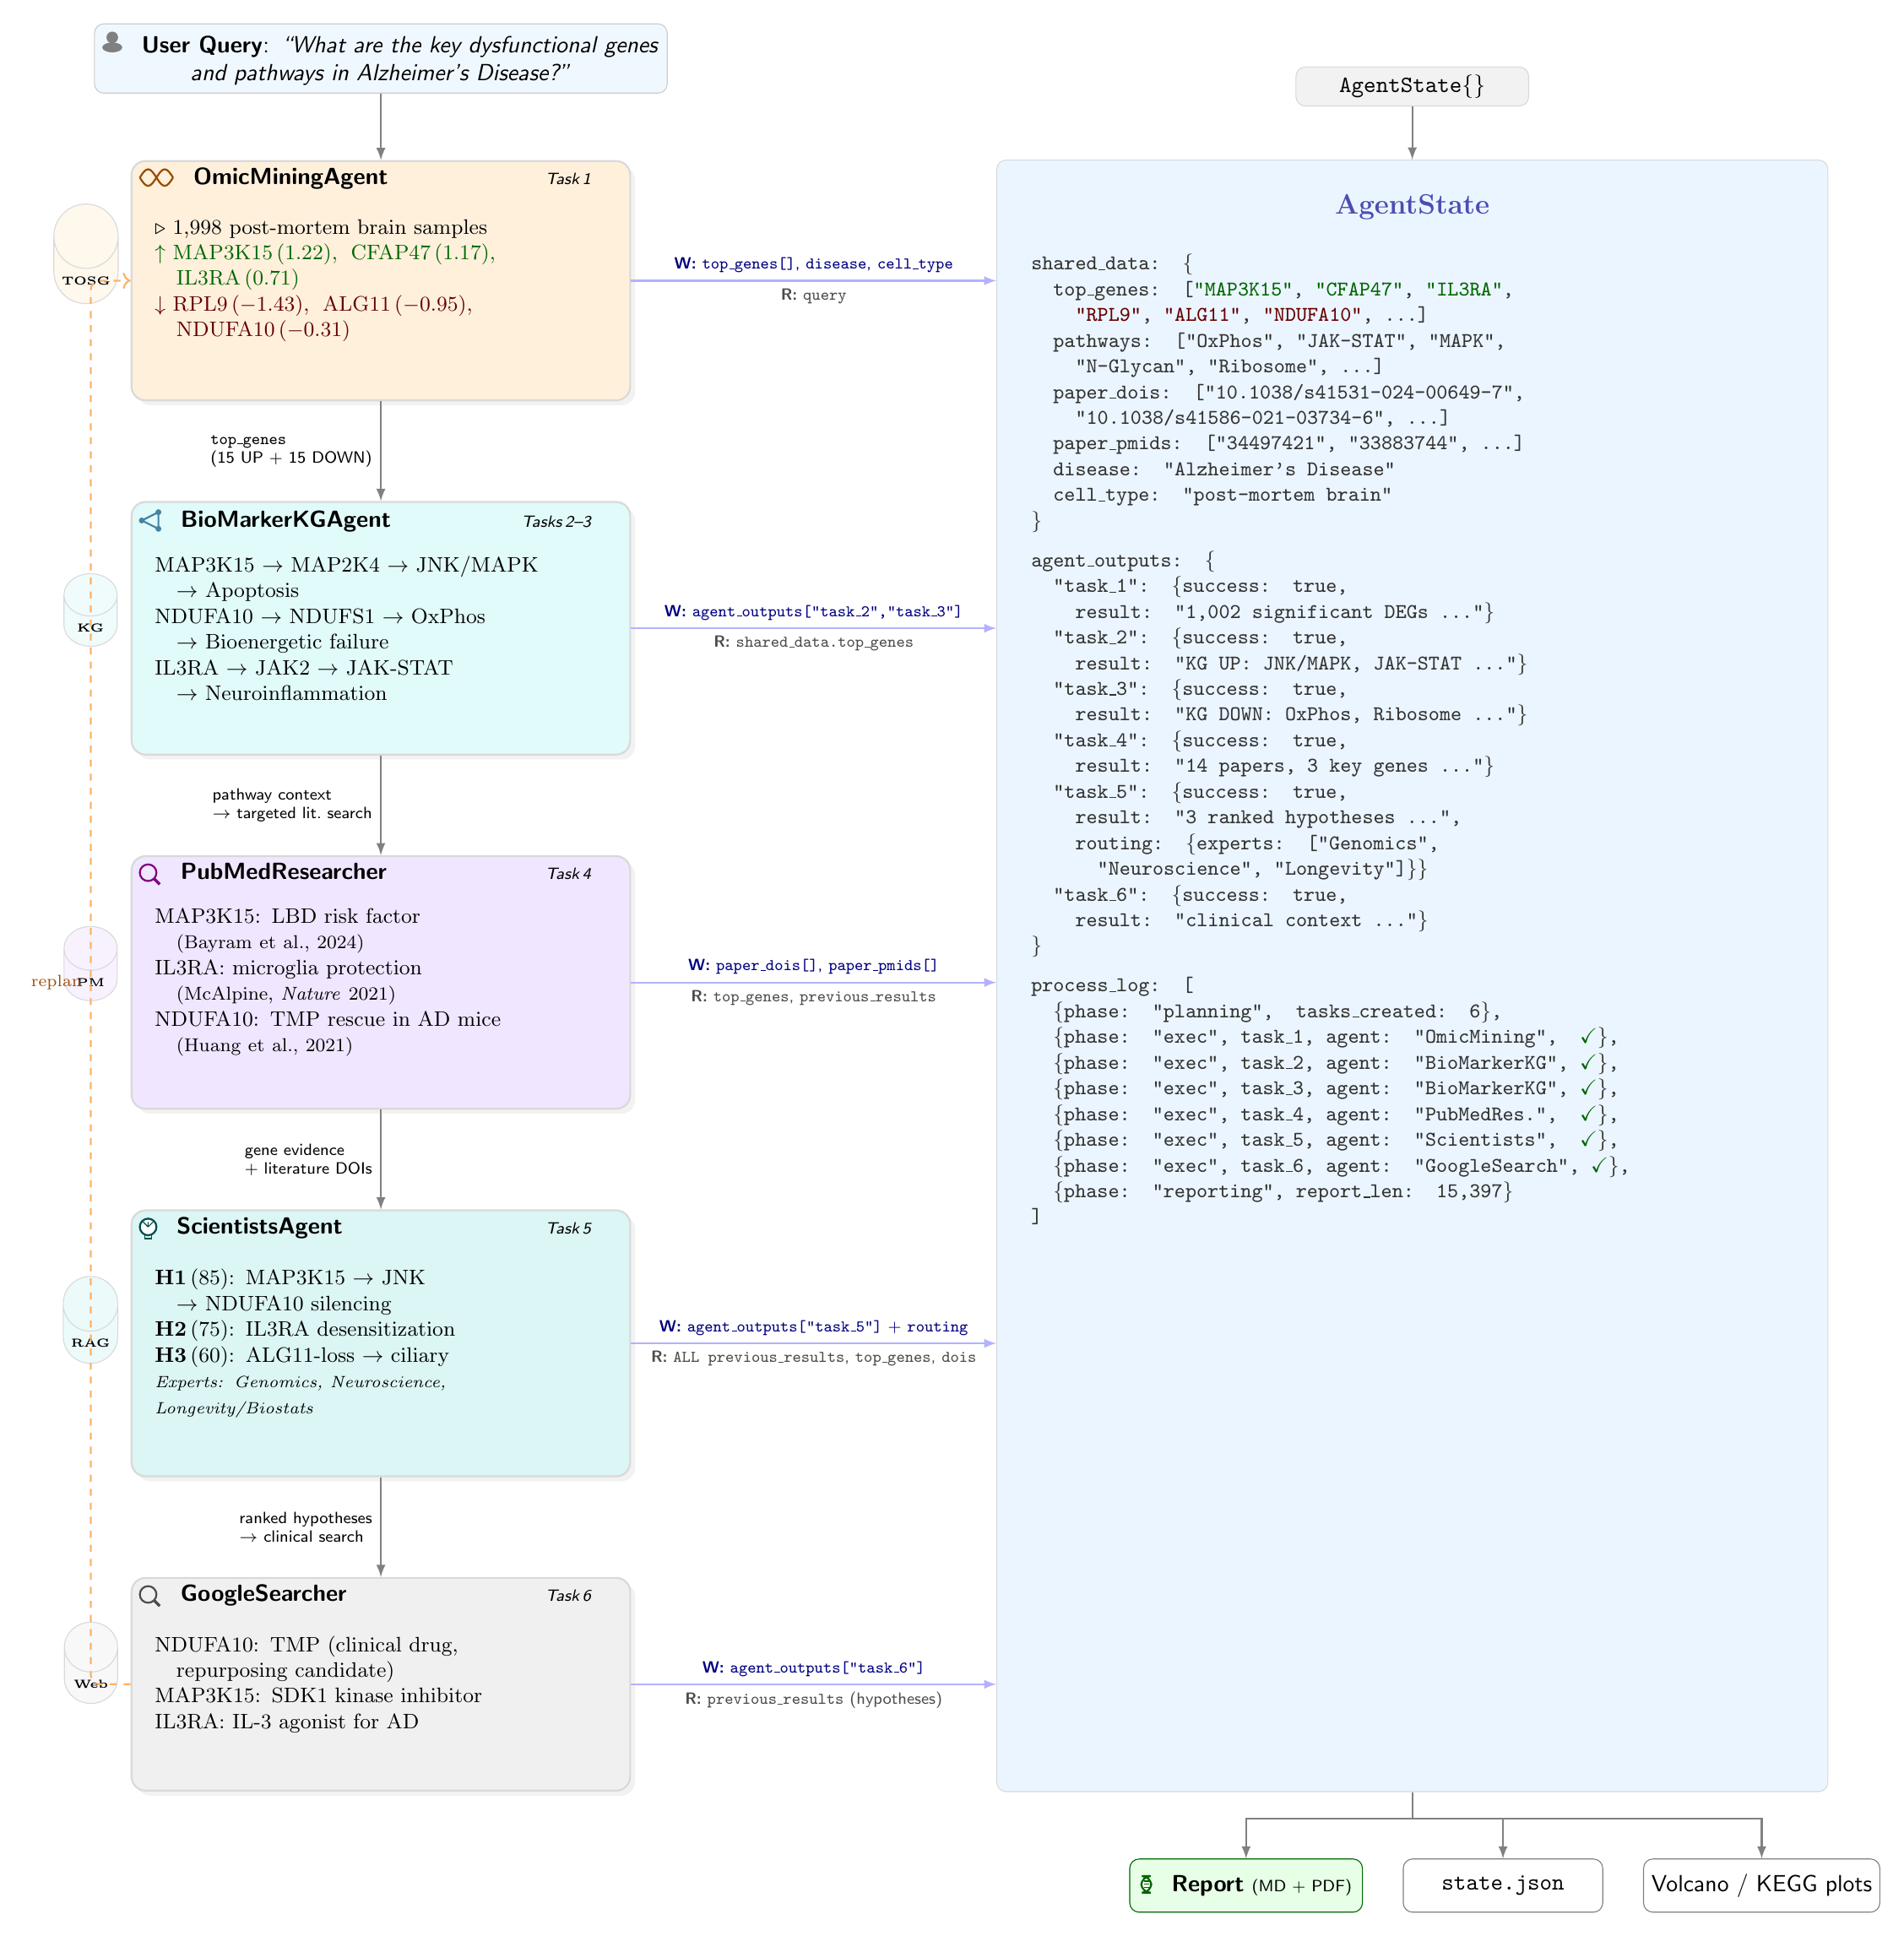
\begin{tikzpicture}[node distance=0.6cm and 1.5cm, font=\sffamily,
        % annotation styles for read/write labels
        wlabel/.style={font=\scriptsize\sffamily, text=blue!50!black, align=left, inner sep=1pt},
        rlabel/.style={font=\scriptsize\sffamily, text=gray!60!black, align=left, inner sep=1pt},
        flowlabel/.style={font=\scriptsize\sffamily, align=left}
    ]

    % ================= LEFT COLUMN: AGENTS =================

    % 1. Input
    \node[draw=gray!40, fill=aliceblue, rounded corners,
          minimum width=6.5cm, minimum height=1.0cm, align=center] (query)
        {\iconUser{gray} \enskip \textbf{User Query}:
         \textit{``What are the key dysfunctional genes}\\
         \textit{and pathways in Alzheimer's Disease?''}};

    % 2. OmicMiningAgent  (Task 1)
    \node[agentbox, fill=agentOrange, minimum height=3.6cm, below=1.0cm of query] (omic) {};
    \node[anchor=north west, text width=6.8cm] at (omic.north west)
        {\iconDNA{orange!60!black} \enskip \textbf{OmicMiningAgent}
         \hfill {\scriptsize\itshape Task\,1}};
    \node[anchor=center, font=\small, align=left, text width=6.8cm] at (omic.center) {
        $\triangleright$ 1{,}998 post-mortem brain samples\\
        \textcolor{green!40!black}{$\uparrow$ MAP3K15\,(1.22),\; CFAP47\,(1.17),}\\
        \textcolor{green!40!black}{\quad IL3RA\,(0.71)}\\
        \textcolor{red!40!black}{$\downarrow$ RPL9\,($-$1.43),\; ALG11\,($-$0.95),}\\
        \textcolor{red!40!black}{\quad NDUFA10\,($-$0.31)}
    };
    \node[database, fill=agentOrange!50, left=0.2cm of omic] (db1) {TOSG};

    % 3. BioMarkerKGAgent  (Tasks 2–3)
    \node[agentbox, fill=agentCyan, minimum height=3.8cm, below=1.5cm of omic] (kg) {};
    \node[anchor=north west, text width=6.8cm] at (kg.north west)
        {\iconGraph{cyan!60!black} \enskip \textbf{BioMarkerKGAgent}
         \hfill {\scriptsize\itshape Tasks\,2--3}};
    \node[anchor=center, font=\small, align=left, text width=6.8cm] at (kg.center) {
        MAP3K15 $\rightarrow$ MAP2K4 $\rightarrow$ JNK/MAPK\\
        \quad $\rightarrow$ Apoptosis\\
        NDUFA10 $\rightarrow$ NDUFS1 $\rightarrow$ OxPhos\\
        \quad $\rightarrow$ Bioenergetic failure\\
        IL3RA $\rightarrow$ JAK2 $\rightarrow$ JAK-STAT\\
        \quad $\rightarrow$ Neuroinflammation
    };
    \node[database, fill=agentCyan!50, left=0.2cm of kg] (db2) {KG};

    % 4. PubMedResearcher  (Task 4)
    \node[agentbox, fill=agentPurple, minimum height=3.8cm, below=1.5cm of kg] (pubmed) {};
    \node[anchor=north west, text width=6.8cm] at (pubmed.north west)
        {\iconSearch{violet} \enskip \textbf{PubMedResearcher}
         \hfill {\scriptsize\itshape Task\,4}};
    \node[anchor=center, font=\small, align=left, text width=6.8cm] at (pubmed.center) {
        MAP3K15: LBD risk factor\\
        \quad {\footnotesize(Bayram et al., 2024)}\\
        IL3RA: microglia protection\\
        \quad {\footnotesize(McAlpine, \textit{Nature} 2021)}\\
        NDUFA10: TMP rescue in AD mice\\
        \quad {\footnotesize(Huang et al., 2021)}
    };
    \node[database, fill=agentPurple!50, left=0.2cm of pubmed] (db3) {PM};

    % 5. ScientistsAgent  (Task 5 — multi-expert)
    \node[agentbox, fill=agentTeal, minimum height=4.0cm, below=1.5cm of pubmed] (scientist) {};
    \node[anchor=north west, text width=6.8cm] at (scientist.north west)
        {\iconBulb{teal!60!black} \enskip \textbf{ScientistsAgent}
         \hfill {\scriptsize\itshape Task\,5}};
    \node[anchor=center, font=\small, align=left, text width=6.8cm] at (scientist.center) {
        \textbf{H1}\,(85): MAP3K15 $\rightarrow$ JNK\\
        \quad $\rightarrow$ NDUFA10 silencing\\
        \textbf{H2}\,(75): IL3RA desensitization\\
        \textbf{H3}\,(60): ALG11-loss $\rightarrow$ ciliary\\
        {\scriptsize\itshape Experts: Genomics, Neuroscience,}\\
        {\scriptsize\itshape Longevity/Biostats}
    };
    \node[database, fill=agentTeal!50, left=0.2cm of scientist] (db4) {RAG};

    % 6. GoogleSearcher  (Task 6)
    \node[agentbox, fill=googleGray, minimum height=3.2cm, below=1.5cm of scientist] (google) {};
    \node[anchor=north west, text width=6.8cm] at (google.north west)
        {\iconSearch{gray!60!black} \enskip \textbf{GoogleSearcher}
         \hfill {\scriptsize\itshape Task\,6}};
    \node[anchor=center, font=\small, align=left, text width=6.8cm] at (google.center) {
        NDUFA10: TMP (clinical drug,\\
        \quad repurposing candidate)\\
        MAP3K15: SDK1 kinase inhibitor\\
        IL3RA: IL-3 agonist for AD
    };
    \node[database, fill=googleGray!50, left=0.2cm of google] (db5) {Web};


    % ================= RIGHT COLUMN: AgentState =================

    \node[draw=gray!30, fill=stateBlue, rounded corners, inner sep=0pt,
          fit={($(omic.north east)+(5.5cm,0)$) ($(google.south east)+(18.0cm,0)$)}]
          (statebox) {};

    % Header
    \node[anchor=north, font=\large\bfseries, color=blue!40!gray, yshift=-0.4cm]
        at (statebox.north) {AgentState};

    % State Content — real AD-test data
    \node[anchor=north west, align=left, font=\ttfamily\small,
          text=gray!40!black] at ($(statebox.north west) + (0.4cm, -1.3cm)$) {%
shared\_data: \{\\
\ \ top\_genes: [%
\textcolor{green!40!black}{"MAP3K15"}, %
\textcolor{green!40!black}{"CFAP47"}, %
\textcolor{green!40!black}{"IL3RA"},\\
\ \ \ \ %
\textcolor{red!40!black}{"RPL9"}, %
\textcolor{red!40!black}{"ALG11"}, %
\textcolor{red!40!black}{"NDUFA10"}, ...]\\
\ \ pathways: ["OxPhos", "JAK-STAT", "MAPK",\\
\ \ \ \ "N-Glycan", "Ribosome", ...]\\
\ \ paper\_dois: ["10.1038/s41531-024-00649-7",\\
\ \ \ \ "10.1038/s41586-021-03734-6", ...]\\
\ \ paper\_pmids: ["34497421", "33883744", ...]\\
\ \ disease: "Alzheimer's Disease"\\
\ \ cell\_type: "post-mortem brain"\\
\}\\[6pt]
agent\_outputs: \{\\
\ \ "task\_1": \{success: true,\\
\ \ \ \ result: "1{,}002 significant DEGs ..."\}\\
\ \ "task\_2": \{success: true,\\
\ \ \ \ result: "KG UP: JNK/MAPK, JAK-STAT ..."\}\\
\ \ "task\_3": \{success: true,\\
\ \ \ \ result: "KG DOWN: OxPhos, Ribosome ..."\}\\
\ \ "task\_4": \{success: true,\\
\ \ \ \ result: "14 papers, 3 key genes ..."\}\\
\ \ "task\_5": \{success: true,\\
\ \ \ \ result: "3 ranked hypotheses ...",\\
\ \ \ \ routing: \{experts: ["Genomics",\\
\ \ \ \ \ \ "Neuroscience", "Longevity"]\}\}\\
\ \ "task\_6": \{success: true,\\
\ \ \ \ result: "clinical context ..."\}\\
\}\\[6pt]
process\_log: [\\
\ \ \{phase: "planning",\ \ tasks\_created: 6\},\\
\ \ \{phase: "exec", task\_1, agent: "OmicMining",\quad \textcolor{green!40!black}{\checkmark}\},\\
\ \ \{phase: "exec", task\_2, agent: "BioMarkerKG",\ \textcolor{green!40!black}{\checkmark}\},\\
\ \ \{phase: "exec", task\_3, agent: "BioMarkerKG",\ \textcolor{green!40!black}{\checkmark}\},\\
\ \ \{phase: "exec", task\_4, agent: "PubMedRes.",\ \ \textcolor{green!40!black}{\checkmark}\},\\
\ \ \{phase: "exec", task\_5, agent: "Scientists",\ \ \textcolor{green!40!black}{\checkmark}\},\\
\ \ \{phase: "exec", task\_6, agent: "GoogleSearch", \textcolor{green!40!black}{\checkmark}\},\\
\ \ \{phase: "reporting", report\_len: 15{,}397\}\\
]
    };

    % Initial State Input
    \node[draw=gray!30, fill=gray!10, rounded corners,
          above=0.8cm of statebox, minimum width=3.5cm] (initstate)
        {\texttt{AgentState\{\}}};
    \draw[->, >=latex, thick, draw=gray] (initstate) -- (statebox);


    % ================= VERTICAL FLOW (data dependencies) =================
    % Labels on LEFT to avoid collision with horizontal read/write annotations

    \draw[->, >=latex, thick, draw=gray] (query) -- (omic);

    \draw[->, >=latex, thick, draw=gray] (omic) --
        node[left, flowlabel]
            {\texttt{top\_genes}\\{\scriptsize(15 UP + 15 DOWN)}} (kg);

    \draw[->, >=latex, thick, draw=gray] (kg) --
        node[left, flowlabel]
            {pathway context\\{\scriptsize$\rightarrow$ targeted lit.\ search}} (pubmed);

    \draw[->, >=latex, thick, draw=gray] (pubmed) --
        node[left, flowlabel]
            {gene evidence\\{\scriptsize+ literature DOIs}} (scientist);

    \draw[->, >=latex, thick, draw=gray] (scientist) --
        node[left, flowlabel]
            {ranked hypotheses\\{\scriptsize$\rightarrow$ clinical search}} (google);


    % ================= HORIZONTAL STATE ARROWS (read/write) =================

    % OmicMiningAgent → State
    \draw[statearrow] (omic.east) -- (omic.east -| statebox.west)
        node[midway, above=2pt, wlabel]
            {\textbf{W:} \texttt{top\_genes[]}, \texttt{disease}, \texttt{cell\_type}}
        node[midway, below=2pt, rlabel]
            {\textbf{R:} \texttt{query}};

    % BioMarkerKGAgent → State
    \draw[statearrow] (kg.east) -- (kg.east -| statebox.west)
        node[midway, above=2pt, wlabel]
            {\textbf{W:} \texttt{agent\_outputs["task\_2","task\_3"]}}
        node[midway, below=2pt, rlabel]
            {\textbf{R:} \texttt{shared\_data.top\_genes}};

    % PubMedResearcher → State
    \draw[statearrow] (pubmed.east) -- (pubmed.east -| statebox.west)
        node[midway, above=2pt, wlabel]
            {\textbf{W:} \texttt{paper\_dois[]}, \texttt{paper\_pmids[]}}
        node[midway, below=2pt, rlabel]
            {\textbf{R:} \texttt{top\_genes}, \texttt{previous\_results}};

    % ScientistsAgent → State
    \draw[statearrow] (scientist.east) -- (scientist.east -| statebox.west)
        node[midway, above=2pt, wlabel]
            {\textbf{W:} \texttt{agent\_outputs["task\_5"]} + \texttt{routing}}
        node[midway, below=2pt, rlabel]
            {\textbf{R:} \texttt{ALL previous\_results}, \texttt{top\_genes}, \texttt{dois}};

    % GoogleSearcher → State
    \draw[statearrow] (google.east) -- (google.east -| statebox.west)
        node[midway, above=2pt, wlabel]
            {\textbf{W:} \texttt{agent\_outputs["task\_6"]}}
        node[midway, below=2pt, rlabel]
            {\textbf{R:} \texttt{previous\_results} (hypotheses)};


    % ================= REPLAN LOOP =================
    \draw[->, dashed, draw=orange!60, thick, rounded corners]
        (google.west) -- ++(-0.6,0) |-
        node[pos=0.25, left, font=\scriptsize, color=orange!60!black] {replan}
        (omic.west);


    % ================= OUTPUTS =================

    \node[draw=green!40!black, fill=agentGreen, rounded corners,
          below=1.0cm of statebox, xshift=-2.5cm,
          minimum width=3.5cm, minimum height=0.8cm] (report)
        {\iconDoc{green!40!black} \enskip \textbf{Report}
         {\scriptsize(MD + PDF)}};

    \node[draw=gray, fill=white, rounded corners,
          right=0.6cm of report,
          minimum width=3.0cm, minimum height=0.8cm] (json)
        {\texttt{state.json}};

    \node[draw=gray, fill=white, rounded corners,
          right=0.6cm of json,
          minimum width=3.0cm, minimum height=0.8cm] (plots)
        {Volcano / KEGG plots};

    \draw[->, >=latex, thick, draw=gray]
        (statebox.south) -- ++(0,-0.4) -| (report.north);
    \draw[->, >=latex, thick, draw=gray]
        (statebox.south) -- ++(0,-0.4) -| (json.north);
    \draw[->, >=latex, thick, draw=gray]
        (statebox.south) -- ++(0,-0.4) -| (plots.north);

    \end{tikzpicture}%
}% end resizebox
\caption{Example agent workflow for an Alzheimer's Disease query using the
OmniCellAgent system.  The Planner decomposes the query into six sequential
tasks; each sub-agent receives the accumulated \texttt{AgentState} and writes
its outputs back.
\textbf{Read/write annotations} on each horizontal arrow show the specific
state fields consumed and produced: OmicMiningAgent populates
\texttt{top\_genes} (1{,}002 DEGs from 1{,}998 post-mortem brain samples),
BioMarkerKGAgent maps those genes to pathways via PrimeKG,
PubMedResearcher adds literature DOIs for the top hits, ScientistsAgent
routes to three domain experts (Genomics, Neuroscience, Longevity/Biostats)
and synthesises ranked mechanistic hypotheses, and GoogleSearcher assesses
translational viability (e.g.\ TMP for NDUFA10 rescue, SDK1 for MAP3K15
inhibition).  The downward arrows indicate how each step leverages results
from the preceding step---enabling progressively deeper reasoning that
mirrors the workflow of a human research team.}
\label{fig:workflow-example}
\end{figure}

% Requires preamble: agentbox, database, statearrow styles;
%   all icon commands; colors agentOrange/Cyan/Purple/Teal,
%   googleGray, stateBlue, aliceblue, agentGreen, \iconDoc.
% ============================================================

\begin{figure}[p]
\centering
\resizebox{\textwidth}{!}{%
    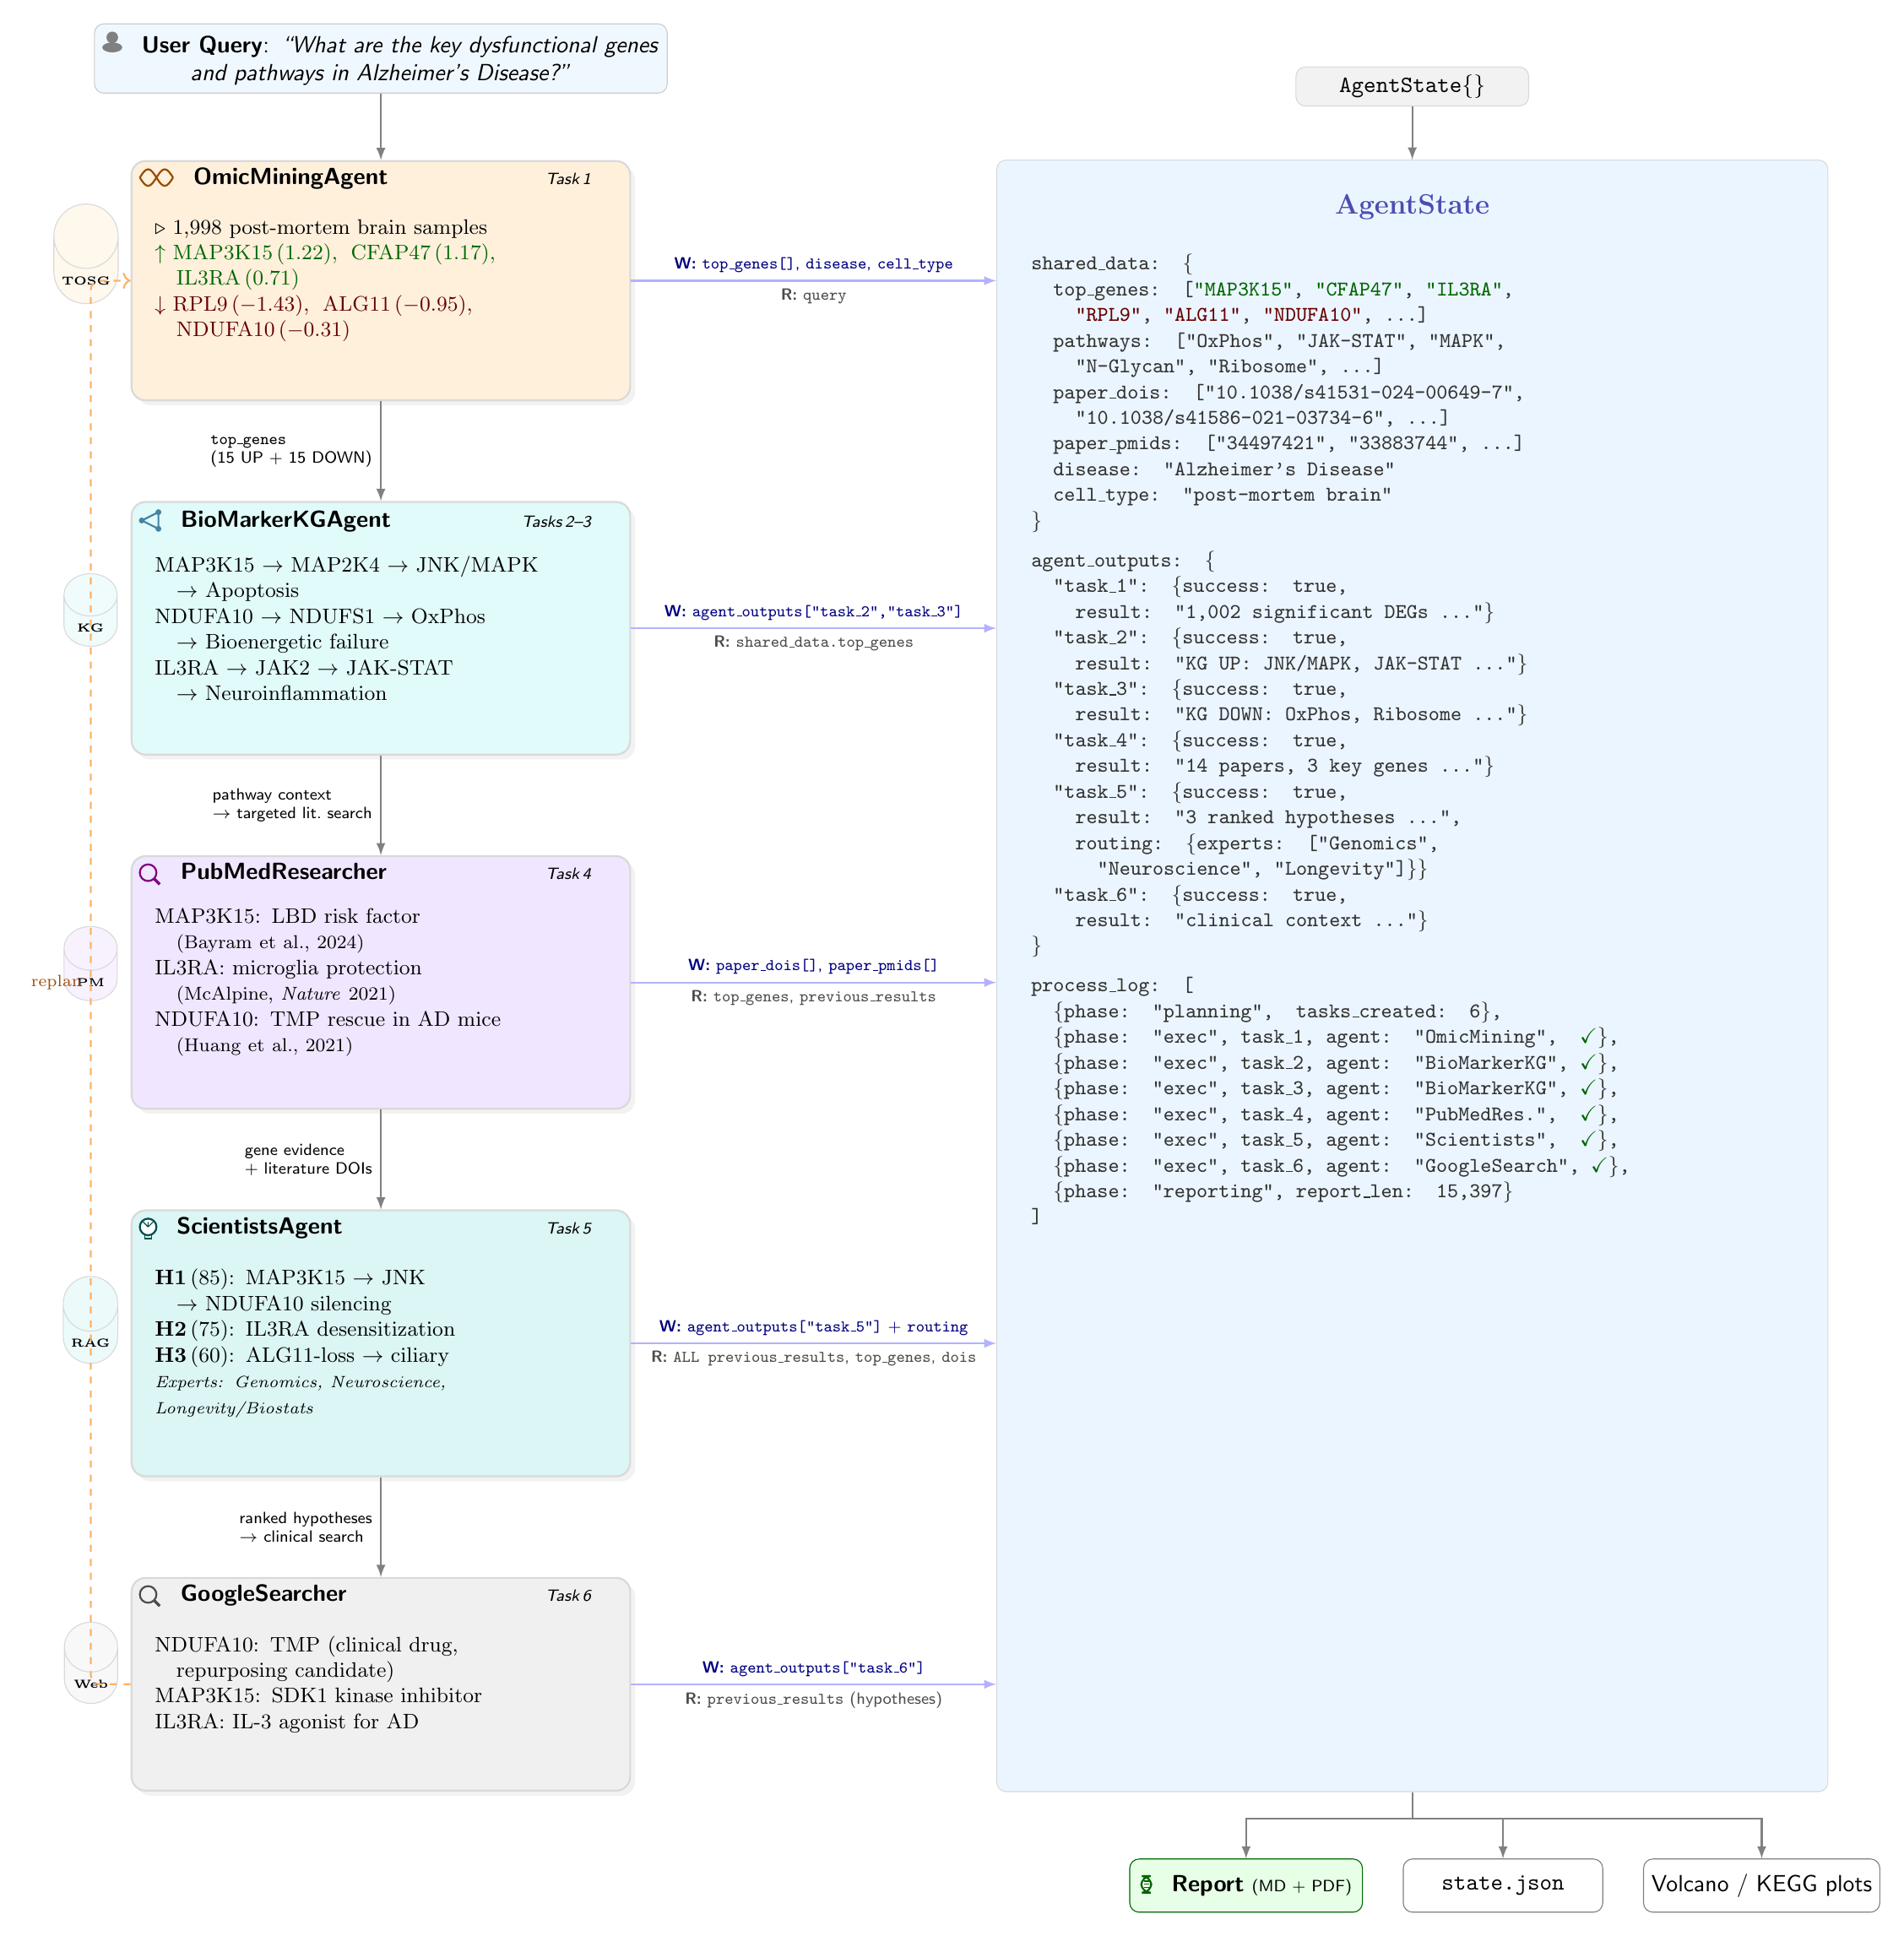
\begin{tikzpicture}[node distance=0.6cm and 1.5cm, font=\sffamily,
        % annotation styles for read/write labels
        wlabel/.style={font=\scriptsize\sffamily, text=blue!50!black, align=left, inner sep=1pt},
        rlabel/.style={font=\scriptsize\sffamily, text=gray!60!black, align=left, inner sep=1pt},
        flowlabel/.style={font=\scriptsize\sffamily, align=left}
    ]

    % ================= LEFT COLUMN: AGENTS =================

    % 1. Input
    \node[draw=gray!40, fill=aliceblue, rounded corners,
          minimum width=6.5cm, minimum height=1.0cm, align=center] (query)
        {\iconUser{gray} \enskip \textbf{User Query}:
         \textit{``What are the key dysfunctional genes}\\
         \textit{and pathways in Alzheimer's Disease?''}};

    % 2. OmicMiningAgent  (Task 1)
    \node[agentbox, fill=agentOrange, minimum height=3.6cm, below=1.0cm of query] (omic) {};
    \node[anchor=north west, text width=6.8cm] at (omic.north west)
        {\iconDNA{orange!60!black} \enskip \textbf{OmicMiningAgent}
         \hfill {\scriptsize\itshape Task\,1}};
    \node[anchor=center, font=\small, align=left, text width=6.8cm] at (omic.center) {
        $\triangleright$ 1{,}998 post-mortem brain samples\\
        \textcolor{green!40!black}{$\uparrow$ MAP3K15\,(1.22),\; CFAP47\,(1.17),}\\
        \textcolor{green!40!black}{\quad IL3RA\,(0.71)}\\
        \textcolor{red!40!black}{$\downarrow$ RPL9\,($-$1.43),\; ALG11\,($-$0.95),}\\
        \textcolor{red!40!black}{\quad NDUFA10\,($-$0.31)}
    };
    \node[database, fill=agentOrange!50, left=0.2cm of omic] (db1) {TOSG};

    % 3. BioMarkerKGAgent  (Tasks 2–3)
    \node[agentbox, fill=agentCyan, minimum height=3.8cm, below=1.5cm of omic] (kg) {};
    \node[anchor=north west, text width=6.8cm] at (kg.north west)
        {\iconGraph{cyan!60!black} \enskip \textbf{BioMarkerKGAgent}
         \hfill {\scriptsize\itshape Tasks\,2--3}};
    \node[anchor=center, font=\small, align=left, text width=6.8cm] at (kg.center) {
        MAP3K15 $\rightarrow$ MAP2K4 $\rightarrow$ JNK/MAPK\\
        \quad $\rightarrow$ Apoptosis\\
        NDUFA10 $\rightarrow$ NDUFS1 $\rightarrow$ OxPhos\\
        \quad $\rightarrow$ Bioenergetic failure\\
        IL3RA $\rightarrow$ JAK2 $\rightarrow$ JAK-STAT\\
        \quad $\rightarrow$ Neuroinflammation
    };
    \node[database, fill=agentCyan!50, left=0.2cm of kg] (db2) {KG};

    % 4. PubMedResearcher  (Task 4)
    \node[agentbox, fill=agentPurple, minimum height=3.8cm, below=1.5cm of kg] (pubmed) {};
    \node[anchor=north west, text width=6.8cm] at (pubmed.north west)
        {\iconSearch{violet} \enskip \textbf{PubMedResearcher}
         \hfill {\scriptsize\itshape Task\,4}};
    \node[anchor=center, font=\small, align=left, text width=6.8cm] at (pubmed.center) {
        MAP3K15: LBD risk factor\\
        \quad {\footnotesize(Bayram et al., 2024)}\\
        IL3RA: microglia protection\\
        \quad {\footnotesize(McAlpine, \textit{Nature} 2021)}\\
        NDUFA10: TMP rescue in AD mice\\
        \quad {\footnotesize(Huang et al., 2021)}
    };
    \node[database, fill=agentPurple!50, left=0.2cm of pubmed] (db3) {PM};

    % 5. ScientistsAgent  (Task 5 — multi-expert)
    \node[agentbox, fill=agentTeal, minimum height=4.0cm, below=1.5cm of pubmed] (scientist) {};
    \node[anchor=north west, text width=6.8cm] at (scientist.north west)
        {\iconBulb{teal!60!black} \enskip \textbf{ScientistsAgent}
         \hfill {\scriptsize\itshape Task\,5}};
    \node[anchor=center, font=\small, align=left, text width=6.8cm] at (scientist.center) {
        \textbf{H1}\,(85): MAP3K15 $\rightarrow$ JNK\\
        \quad $\rightarrow$ NDUFA10 silencing\\
        \textbf{H2}\,(75): IL3RA desensitization\\
        \textbf{H3}\,(60): ALG11-loss $\rightarrow$ ciliary\\
        {\scriptsize\itshape Experts: Genomics, Neuroscience,}\\
        {\scriptsize\itshape Longevity/Biostats}
    };
    \node[database, fill=agentTeal!50, left=0.2cm of scientist] (db4) {RAG};

    % 6. GoogleSearcher  (Task 6)
    \node[agentbox, fill=googleGray, minimum height=3.2cm, below=1.5cm of scientist] (google) {};
    \node[anchor=north west, text width=6.8cm] at (google.north west)
        {\iconSearch{gray!60!black} \enskip \textbf{GoogleSearcher}
         \hfill {\scriptsize\itshape Task\,6}};
    \node[anchor=center, font=\small, align=left, text width=6.8cm] at (google.center) {
        NDUFA10: TMP (clinical drug,\\
        \quad repurposing candidate)\\
        MAP3K15: SDK1 kinase inhibitor\\
        IL3RA: IL-3 agonist for AD
    };
    \node[database, fill=googleGray!50, left=0.2cm of google] (db5) {Web};


    % ================= RIGHT COLUMN: AgentState =================

    \node[draw=gray!30, fill=stateBlue, rounded corners, inner sep=0pt,
          fit={($(omic.north east)+(5.5cm,0)$) ($(google.south east)+(18.0cm,0)$)}]
          (statebox) {};

    % Header
    \node[anchor=north, font=\large\bfseries, color=blue!40!gray, yshift=-0.4cm]
        at (statebox.north) {AgentState};

    % State Content — real AD-test data
    \node[anchor=north west, align=left, font=\ttfamily\small,
          text=gray!40!black] at ($(statebox.north west) + (0.4cm, -1.3cm)$) {%
shared\_data: \{\\
\ \ top\_genes: [%
\textcolor{green!40!black}{"MAP3K15"}, %
\textcolor{green!40!black}{"CFAP47"}, %
\textcolor{green!40!black}{"IL3RA"},\\
\ \ \ \ %
\textcolor{red!40!black}{"RPL9"}, %
\textcolor{red!40!black}{"ALG11"}, %
\textcolor{red!40!black}{"NDUFA10"}, ...]\\
\ \ pathways: ["OxPhos", "JAK-STAT", "MAPK",\\
\ \ \ \ "N-Glycan", "Ribosome", ...]\\
\ \ paper\_dois: ["10.1038/s41531-024-00649-7",\\
\ \ \ \ "10.1038/s41586-021-03734-6", ...]\\
\ \ paper\_pmids: ["34497421", "33883744", ...]\\
\ \ disease: "Alzheimer's Disease"\\
\ \ cell\_type: "post-mortem brain"\\
\}\\[6pt]
agent\_outputs: \{\\
\ \ "task\_1": \{success: true,\\
\ \ \ \ result: "1{,}002 significant DEGs ..."\}\\
\ \ "task\_2": \{success: true,\\
\ \ \ \ result: "KG UP: JNK/MAPK, JAK-STAT ..."\}\\
\ \ "task\_3": \{success: true,\\
\ \ \ \ result: "KG DOWN: OxPhos, Ribosome ..."\}\\
\ \ "task\_4": \{success: true,\\
\ \ \ \ result: "14 papers, 3 key genes ..."\}\\
\ \ "task\_5": \{success: true,\\
\ \ \ \ result: "3 ranked hypotheses ...",\\
\ \ \ \ routing: \{experts: ["Genomics",\\
\ \ \ \ \ \ "Neuroscience", "Longevity"]\}\}\\
\ \ "task\_6": \{success: true,\\
\ \ \ \ result: "clinical context ..."\}\\
\}\\[6pt]
process\_log: [\\
\ \ \{phase: "planning",\ \ tasks\_created: 6\},\\
\ \ \{phase: "exec", task\_1, agent: "OmicMining",\quad \textcolor{green!40!black}{\checkmark}\},\\
\ \ \{phase: "exec", task\_2, agent: "BioMarkerKG",\ \textcolor{green!40!black}{\checkmark}\},\\
\ \ \{phase: "exec", task\_3, agent: "BioMarkerKG",\ \textcolor{green!40!black}{\checkmark}\},\\
\ \ \{phase: "exec", task\_4, agent: "PubMedRes.",\ \ \textcolor{green!40!black}{\checkmark}\},\\
\ \ \{phase: "exec", task\_5, agent: "Scientists",\ \ \textcolor{green!40!black}{\checkmark}\},\\
\ \ \{phase: "exec", task\_6, agent: "GoogleSearch", \textcolor{green!40!black}{\checkmark}\},\\
\ \ \{phase: "reporting", report\_len: 15{,}397\}\\
]
    };

    % Initial State Input
    \node[draw=gray!30, fill=gray!10, rounded corners,
          above=0.8cm of statebox, minimum width=3.5cm] (initstate)
        {\texttt{AgentState\{\}}};
    \draw[->, >=latex, thick, draw=gray] (initstate) -- (statebox);


    % ================= VERTICAL FLOW (data dependencies) =================
    % Labels on LEFT to avoid collision with horizontal read/write annotations

    \draw[->, >=latex, thick, draw=gray] (query) -- (omic);

    \draw[->, >=latex, thick, draw=gray] (omic) --
        node[left, flowlabel]
            {\texttt{top\_genes}\\{\scriptsize(15 UP + 15 DOWN)}} (kg);

    \draw[->, >=latex, thick, draw=gray] (kg) --
        node[left, flowlabel]
            {pathway context\\{\scriptsize$\rightarrow$ targeted lit.\ search}} (pubmed);

    \draw[->, >=latex, thick, draw=gray] (pubmed) --
        node[left, flowlabel]
            {gene evidence\\{\scriptsize+ literature DOIs}} (scientist);

    \draw[->, >=latex, thick, draw=gray] (scientist) --
        node[left, flowlabel]
            {ranked hypotheses\\{\scriptsize$\rightarrow$ clinical search}} (google);


    % ================= HORIZONTAL STATE ARROWS (read/write) =================

    % OmicMiningAgent → State
    \draw[statearrow] (omic.east) -- (omic.east -| statebox.west)
        node[midway, above=2pt, wlabel]
            {\textbf{W:} \texttt{top\_genes[]}, \texttt{disease}, \texttt{cell\_type}}
        node[midway, below=2pt, rlabel]
            {\textbf{R:} \texttt{query}};

    % BioMarkerKGAgent → State
    \draw[statearrow] (kg.east) -- (kg.east -| statebox.west)
        node[midway, above=2pt, wlabel]
            {\textbf{W:} \texttt{agent\_outputs["task\_2","task\_3"]}}
        node[midway, below=2pt, rlabel]
            {\textbf{R:} \texttt{shared\_data.top\_genes}};

    % PubMedResearcher → State
    \draw[statearrow] (pubmed.east) -- (pubmed.east -| statebox.west)
        node[midway, above=2pt, wlabel]
            {\textbf{W:} \texttt{paper\_dois[]}, \texttt{paper\_pmids[]}}
        node[midway, below=2pt, rlabel]
            {\textbf{R:} \texttt{top\_genes}, \texttt{previous\_results}};

    % ScientistsAgent → State
    \draw[statearrow] (scientist.east) -- (scientist.east -| statebox.west)
        node[midway, above=2pt, wlabel]
            {\textbf{W:} \texttt{agent\_outputs["task\_5"]} + \texttt{routing}}
        node[midway, below=2pt, rlabel]
            {\textbf{R:} \texttt{ALL previous\_results}, \texttt{top\_genes}, \texttt{dois}};

    % GoogleSearcher → State
    \draw[statearrow] (google.east) -- (google.east -| statebox.west)
        node[midway, above=2pt, wlabel]
            {\textbf{W:} \texttt{agent\_outputs["task\_6"]}}
        node[midway, below=2pt, rlabel]
            {\textbf{R:} \texttt{previous\_results} (hypotheses)};


    % ================= REPLAN LOOP =================
    \draw[->, dashed, draw=orange!60, thick, rounded corners]
        (google.west) -- ++(-0.6,0) |-
        node[pos=0.25, left, font=\scriptsize, color=orange!60!black] {replan}
        (omic.west);


    % ================= OUTPUTS =================

    \node[draw=green!40!black, fill=agentGreen, rounded corners,
          below=1.0cm of statebox, xshift=-2.5cm,
          minimum width=3.5cm, minimum height=0.8cm] (report)
        {\iconDoc{green!40!black} \enskip \textbf{Report}
         {\scriptsize(MD + PDF)}};

    \node[draw=gray, fill=white, rounded corners,
          right=0.6cm of report,
          minimum width=3.0cm, minimum height=0.8cm] (json)
        {\texttt{state.json}};

    \node[draw=gray, fill=white, rounded corners,
          right=0.6cm of json,
          minimum width=3.0cm, minimum height=0.8cm] (plots)
        {Volcano / KEGG plots};

    \draw[->, >=latex, thick, draw=gray]
        (statebox.south) -- ++(0,-0.4) -| (report.north);
    \draw[->, >=latex, thick, draw=gray]
        (statebox.south) -- ++(0,-0.4) -| (json.north);
    \draw[->, >=latex, thick, draw=gray]
        (statebox.south) -- ++(0,-0.4) -| (plots.north);

    \end{tikzpicture}%
}% end resizebox
\caption{Example agent workflow for an Alzheimer's Disease query using the
OmniCellAgent system.  The Planner decomposes the query into six sequential
tasks; each sub-agent receives the accumulated \texttt{AgentState} and writes
its outputs back.
\textbf{Read/write annotations} on each horizontal arrow show the specific
state fields consumed and produced: OmicMiningAgent populates
\texttt{top\_genes} (1{,}002 DEGs from 1{,}998 post-mortem brain samples),
BioMarkerKGAgent maps those genes to pathways via PrimeKG,
PubMedResearcher adds literature DOIs for the top hits, ScientistsAgent
routes to three domain experts (Genomics, Neuroscience, Longevity/Biostats)
and synthesises ranked mechanistic hypotheses, and GoogleSearcher assesses
translational viability (e.g.\ TMP for NDUFA10 rescue, SDK1 for MAP3K15
inhibition).  The downward arrows indicate how each step leverages results
from the preceding step---enabling progressively deeper reasoning that
mirrors the workflow of a human research team.}
\label{fig:workflow-example}
\end{figure}

\end{document}
